\documentclass[a4paper,12pt]{article}
\usepackage[utf8]{inputenc}
\usepackage{graphicx}
\usepackage{amsmath}
\usepackage{amsfonts}
\usepackage{amssymb}
\usepackage{hyperref}
\usepackage{float}
\usepackage{geometry}
\usepackage{tabto}
\geometry{margin=1in}
\usepackage{csquotes}
\usepackage{listings}
\usepackage{xcolor} 
\usepackage{tcolorbox}


\lstset{
    language=Matlab, % The language of the code
    basicstyle=\ttfamily\small, % The basic font style used
    keywordstyle=\color{blue}\bfseries, % Style for keywords
    commentstyle=\color{green}, % Style for comments
    stringstyle=\color{red}, % Style for strings
    numbers=left, % Where to put line numbers
    numberstyle=\small\color{gray}, % Style for line numbers
    stepnumber=1, % Line number step size
    numbersep=10pt, % Space between line numbers and code
    backgroundcolor=\color{lightgray!10}, % Background color for the code block
    frame=single, % Frame around the code block
    breaklines=true, % Automatic line breaking
    captionpos=b % Caption position (b for bottom, t for top)
}

\tcbset{
  observation/.style={
    colback=yellow!10!white, % Background color
    colframe=black, % Border color
    fonttitle=\bfseries, % Title font
    coltitle=black, % Title color
    boxrule=0.5mm, % Border thickness
    title=Observation, % Title text
    sharp corners, % Sharp corners
    enhanced, % Allows more features
    attach boxed title to top left={yshift=-2mm, xshift=2mm},
    boxed title style={colframe=black, colback=yellow!30!white, boxrule=0.5mm},
  }
}


\tcbset{
  mybox/.style={
    colback=blue!5!white, % Background color
    colframe=blue!75!black, % Border color
    fonttitle=\bfseries, % Title font style
    boxrule=0.5mm, % Border thickness
    sharp corners, % Sharp corners
    enhanced, % Enhanced features
  }
}


\tcbset{
  historicalbox/.style={
    colback=yellow!10!white, % Background color
    colframe=orange!85!black, % Border color
    fonttitle=\bfseries, % Title font style
    title=Historical Curiosity, % Title of the box
    boxrule=1mm, % Border thickness
    sharp corners, % Sharp corners for the box
    enhanced, % Allows for more features
    coltitle=black, % Title color
    left=2mm, right=2mm, top=2mm, bottom=2mm, % Padding
    width=\textwidth, % Box width
    arc=2mm, % Corner rounding
  }
}




\title{Control of Cyber-physical Systems\\ \vspace{0.5cm} \large LABORATORY WORK REPORT | PART I\\ \vspace{0.5cm} \large Identification of a Flexible Robot Arm Joint\begin{center}
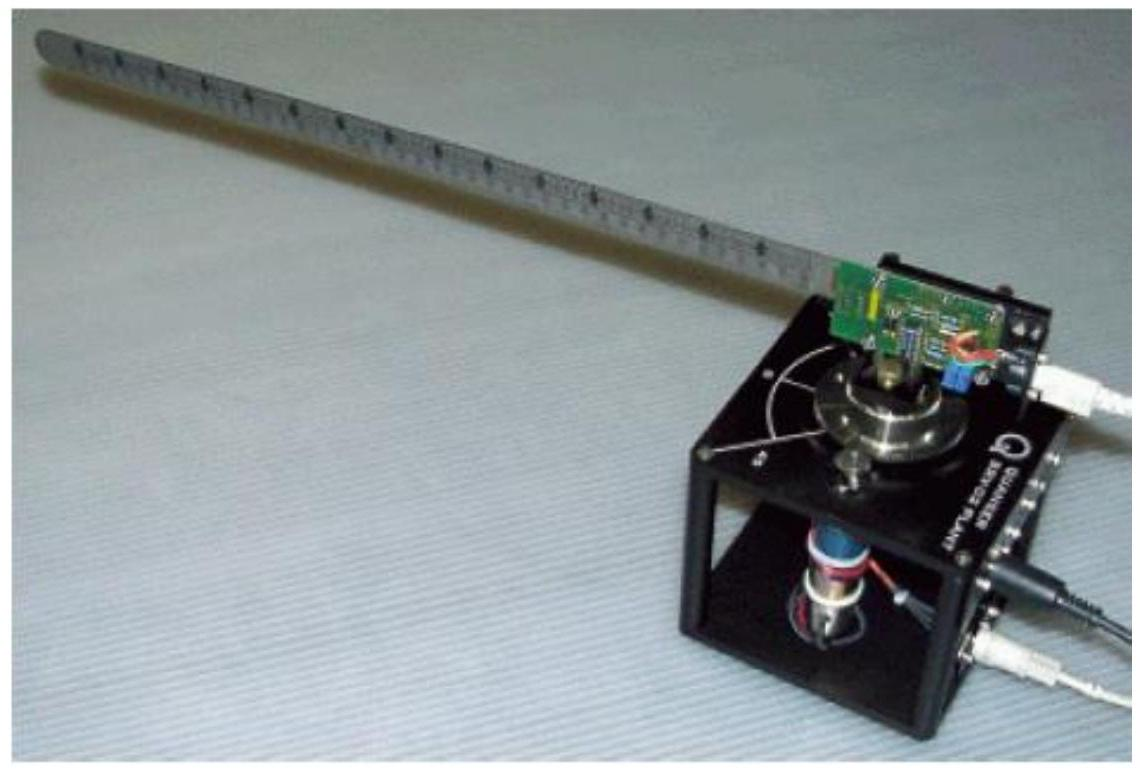
\includegraphics[width=0.6\textwidth]{Figs/2024_08_29_9e657742dc855ba919cag-01}

\vspace{15pt}
\emph{Shift X} %% insert here the number of the shift you have attended
\end{center}}

\author{ \emph{Group XX}: %% insert here the group number
    \\ \tabto{0.1cm}Name Surname | XXXXXX    %% insert here the name, surname, and IST student number of each group member
    \\ \tabto{0.1cm}Name Surname | XXXXXX
    \\ \tabto{0.1cm}Name Surname | XXXXXX
}
\date{\textbf{2024/2025 – 1st Quarter}}

\begin{document}


\begin{figure}[t]
    \flushleft
    
\includegraphics[width=5cm]{Figs/IST_A_CMYK_POS.eps} 
\end{figure}

\maketitle
\begin{center}
\textbf{Instituto Superior Técnico\\ Department of Electrical and Computer Engineering\\ Scientific Area of Systems, Decision, and Control}
\end{center}
\vspace{20pt}
\textcolor{red}{\textbf{Important notice:} Please note that you are allowed to add a maximum of 6 pages of content to the current template. The final compiled report, including all sections, shall not exceed 10 pages in total (after compilation into PDF format). Additional pages will not be considered for evaluation.}






\newpage
\tableofcontents
\newpage


\addcontentsline{toc}{section}{{Introduction}}
\section*{Introduction}
\label{sec:intro}

%% Write a small introduction to the first part of this laboratory work

\section{Question 1 - Analyzing the problem (2.5\,pts)}
\label{sec:q1}

\subsection{Why is achieving this control objective nontrivial? (2.5\,pts)}
(\textit{Hints: Is it feasible to create a lookup table of electric voltages for the DC motor that ensures the bar tip remains at a fixed position? What would be the result if a constant voltage is applied to the motor? What would be the result if a constant voltage is applied to the motor? Reflect on the dynamics of the motor and the bar. What might the approximate open-loop pole distribution of the system look like?})
\vspace{15pt}

%%Write your answer here


\section{Question 2 - Interfacing the plant with the computer (5\,pts)}
\label{sec:q2}

\subsection{Comment on the motor operation. Explain in particular why their angular position never stabilizes when its command signal is constant in the open loop conditions described. (0.5\,pts)}
\vspace{10pt}

%%Write your answer here

\subsection{Explain the procedure carried out to perform sensor calibration. (4.5\,pts)}
(\textit{Check the laboratory work guide to see what you should include in this answer.}) 
\vspace{15pt}

%%Write your answer here

\section{Question 3 - Model identification and validation (9.5\,pts)}
\label{sec:q3}

\subsection{Explanation on the tests performed on the plant to obtain the data used for identification. Discuss the results obtained with different types of excitation signals and the effect of very small amplitude and very large amplitude excitation signals. (2\,pts)}
\vspace{10pt}

%%Write your answer here

\subsection{Discussion of the sampling frequency. (1\,pt)}
\vspace{10pt}

%%Write your answer here

\subsection{Effect on identification of filtering the data. (1\,pt)}
\vspace{10pt}

%%Write your answer here

\subsection{Explanation on how the pole at the origin has been dwelt with. (0.5\,pts)}
\vspace{10pt}

%%Write your answer here

\subsection{Discussion on how the model orders have been decided. Take into consideration that the plant results from the interconnection of a DC motor and the flexible bar and discuss the models needed for each of them. (1\,pt)}
\vspace{10pt}

%%Write your answer here

\subsection{Description of the final ARMAX model. (0.5\,pt)}
\vspace{10pt}

%%Write your answer here

\subsection{Description of the final state-space model. (0.5\,pts)}
\vspace{10pt}

%%Write your answer here

\subsection{Characterization of the plant open loop pole-zero plot, frequency response and time response of the model. (1.5\,pt)}
\vspace{10pt}

%%Write your answer here

\subsection{Model validation. (1.5\,pts)}
\vspace{10pt}

%%Write your answer here

\addcontentsline{toc}{section}{{Conclusions}}
\section*{Conclusions}

%% Draw some conclusions about the first part of this laboratory work




\end{document}